% Load float before the class loads hyperref, avoiding duplicate float anchors.
\RequirePackage{float}
\documentclass[a4paper,fleqn]{cas-sc}

\usepackage[authoryear]{natbib}
\usepackage{amsmath,amssymb}
\usepackage{booktabs}
\usepackage{threeparttable}
\usepackage{graphicx}
\usepackage{multirow}
\usepackage{lineno}
\usepackage[section]{placeins}
\usepackage{xcolor}
\usepackage{setspace}
\setlength{\footnotemargin}{0pt}

\ExplSyntaxOn
\cs_new_eq:NN \lr_cusum_original_make_tbl_caption:nn \__make_tbl_caption:nn
\cs_set:Npn \__make_tbl_caption:nn #1#2
  {
    \group_begin:
      \skip_set:Nn \l_tbl_abovecap_skip {3pt}
      \setstretch{1.5}
      \lr_cusum_original_make_tbl_caption:nn {#1} {#2}
    \group_end:
  }
\cs_new_eq:NN \lr_cusum_original_make_fig_caption:nn \__make_fig_caption:nn
\cs_set:Npn \__make_fig_caption:nn #1#2
  {
    \group_begin:
      \skip_set:Nn \l_fig_abovecap_skip {3pt}
      \setstretch{1.5}
      \lr_cusum_original_make_fig_caption:nn {#1} {#2}
    \group_end:
  }
\ExplSyntaxOff

\begin{document}
\linenumbers

\let\WriteBookmarks\relax
\def\floatpagepagefraction{1}
\def\textpagefraction{.001}

\shorttitle{Mapping rotational harvesting in Ecuadorian balsa plantations}
\shortauthors{Rao et al.}

\author[1]{Keyi Rao}[orcid=0000-0001-8443-9819]\fnmark[1]
\credit{Conceptualization, Methodology, Software, Validation, Visualization, Data curation, Formal analysis, Project administration, Writing -- original draft}

\author[1]{Shixin Dong}[orcid=0009-0005-7299-5312]\fnmark[1]
\credit{Methodology, Software, Validation, Writing -- original draft}

\author[2]{Zhongwen Hu}[orcid=0000-0003-2689-3196]
\credit{Validation, Funding acquisition, Writing -- review and editing}

\author[3,4]{Cesar Ivan Alvarez}[orcid=0000-0001-5629-0893]
\credit{Resources, Methodology, Validation}

\author[5]{Yuanyong Dian}[orcid=0000-0002-4957-3681]
\credit{Validation, Writing -- review and editing}

\author[1]{Ruixin Fang}[orcid=0000-0002-1429-632X]
\credit{Validation, Data curation, Software}

\author[1]{Zhaocong Wu}[orcid=0000-0003-2435-5538]\cormark[1]
\ead{zcwoo@whu.edu.cn}
\credit{Conceptualization, Resources, Supervision, Funding acquisition}

\affiliation[1]{organization={School of Remote Sensing and Information Engineering, Wuhan University},
  addressline={No. 299 Bayi Road, Wuchang District}, city={Wuhan}, postcode={430072},
  state={Hubei}, country={China}}
\affiliation[2]{organization={School of Architecture and Urban Planning and MNR Key Laboratory for Geo-Environmental Monitoring of Great Bay Area, Shenzhen University},
  addressline={No. 3688 Nanhai Avenue, Nanshan District}, city={Shenzhen},
  postcode={518060}, state={Guangdong}, country={China}}
\affiliation[3]{organization={College of Horticulture and Forestry Sciences, Huazhong Agricultural University},
  addressline={No. 1 Shizishan Street, Hongshan District}, city={Wuhan}, postcode={430070},
  state={Hubei}, country={China}}
\affiliation[4]{organization={Institute of Geography, Faculty of Applied Informatics, University of Augsburg},
  addressline={Universit\"atsstra\ss e 12}, city={Augsburg}, postcode={86159}, country={Germany}}
\affiliation[5]{organization={Maestr\'ia en Sistemas de Informaci\'on Geogr\'afica, Topograf\'ia Automatizada y Fotogrametr\'ia Digital, Universidad Cat\'olica de Santiago de Guayaquil},
  city={Guayaquil}, country={Ecuador}}

\cortext[cor1]{Corresponding author}
\fntext[fn1]{These authors contributed equally to this work.}

\title[mode=title]{Mapping rotational harvesting from decadal Sentinel-1 time series with windowed CuSum: A case study of Ecuadorian balsa plantations}

\begin{abstract}
  Balsa (\textit{Ochroma pyramidale}) plantations supply lightweight material for wind-turbine blades, but tropical cloud cover obscures their short harvest--regrowth cycles in optical imagery. We developed a retrospective framework to reconstruct stand-level rotational harvest histories from decadal Sentinel-1 synthetic aperture radar (SAR) observations. Track-consistent monthly trajectories at fixed 30~m pixels support windowed CuSum detection, which combines locally renewed baselines, central decision intervals, and window-specific permutation testing. Spatiotemporal aggregation consolidates staggered detections into harvest events and resolves progression within events. Reference-aligned observations showed median post-harvest declines of 1.45~dB in VV and 1.40~dB in VH despite overlapping pooled backscatter distributions. Against 1,049 reference harvests from 459 Ecuadorian stands, windowed CuSum achieved the highest F1 (0.837; precision: 0.782, recall: 0.901) among 14 benchmark configurations. It outperformed adapted ReCuSum (0.789) and CCDC (0.734), raising adjacent harvest-pair recovery from 65.6\% for adapted ReCuSum to 83.9\%, with similar dating accuracy on shared events. Across 3,364 evaluable stands, the framework identified 6,303 harvests during 2017--2025. Repeated harvesting occurred in 59.6\% of stands, with a 34-month median inter-harvest interval. Five cantons accounted for 67.6\% of harvests, and annual activity peaked in 2022. These findings show how decadal SAR archives can recover recurrent canopy turnover and support plantation monitoring in persistently cloudy tropical regions.
\end{abstract}

\begin{highlights}
  \item Decadal Sentinel-1 SAR reconstructs monthly multi-rotation balsa harvest histories
  \item Local baseline adaptation enables recurrent harvest detection in evolving backgrounds
  \item Spatiotemporal aggregation links staggered pixel detections to stand harvests
  \item Windowed CuSum tops 14 detectors (0.837 F1) and recovers 83.9\% of harvest pairs
  \item 59.6\% of Ecuadorian stands showed rotational harvesting (34-month median interval)
\end{highlights}

\begin{keywords}
  Synthetic aperture radar (SAR) \sep
  Change-point detection \sep
  Spatiotemporal aggregation \sep
  Short-rotation plantation \sep
  Stand turnover \sep
  \textit{Ochroma pyramidale}
\end{keywords}

\maketitle
\doublespacing

% !TeX root = ../main.tex
\section{Introduction}
\label{sec:introduction}

Rotational plantation management alternates timber harvesting with rapid regeneration and stand growth. Beyond static maps of plantation extent, reliable records of harvest timing, frequency, and inter-harvest intervals are essential for tracking timber supply across rotations~\citep{McMahon2019EucalyptusRotations} and guiding sustainable plantation management~\citep{Cortes2023PlantationHarvesting}. This temporal dimension is particularly critical for Ecuador's commercial balsa (\textit{Ochroma pyramidale}) plantations. Combining exceptionally low wood density with high specific strength, balsa serves as a primary core material in wind-turbine blades and lightweight composite structures~\citep{Borrega2015Balsa_mechanics}. On productive lowland sites, trees reach merchantable size within roughly three years~\citep{CanadasLopez2019BalsaGrowth}, enabling multiple harvest--regrowth cycles on the same parcel within a single decade. Because single-date inventories cannot capture this turnover and sparse observations readily miss harvests obscured by rapid canopy closure~\citep{Huang2026EucalyptusAge}, sustained, high-frequency satellite time series are required to reconstruct rotational harvesting histories.

Long-term optical time-series algorithms such as LandTrendr and CCDC have widely enabled forest disturbance and plantation age reconstruction where clear-sky imagery is abundant~\citep{Kennedy2010LandTrendr,Zhu2014CCDC,Huang2026EucalyptusAge}. Resolving successive short rotations, however, requires uninterrupted observations spanning both canopy removal and intervening regrowth. Across humid tropical regions, persistent cloud cover creates prolonged data gaps~\citep{FloresAnderson2023TropicalCloudFreeOptical}. In mainland Ecuador, year-round cloudiness and cirrus contamination severely restrict usable optical imagery, often forcing regional studies to rely on multi-year optical composites~\citep{OchoaBrito2023EcuadorCropland,AlvarezMendoza2019CirrusEcuador} that sacrifice the monthly precision needed to date individual harvests. Optical archives alone therefore remain insufficient for reconstructing multi-rotation balsa harvest histories.

Sentinel-1 C-band synthetic aperture radar (SAR) overcomes cloud constraints by providing dense, all-weather observations sensitive to canopy geometry and dielectric structure~\citep{Torres2012S1,Reiche2021CongoAlerts}. In short-rotation plantations, clear-felling reduces co- and cross-polarized backscatter, followed by progressive recovery as young stands regenerate~\citep{Spracklen2021Acacia}. Building on this physical response, dense Sentinel-1 time series have supported tropical disturbance alerts, continuous change monitoring, and monthly harvest mapping~\citep{Reiche2021CongoAlerts,Bullock2022CCDC_S1,Zhao2022MonthlyHarvest,Balling2023Texture}.

Extending SAR disturbance detection from isolated alerts to decadal, multi-rotation harvest histories nevertheless faces three distinct challenges. First, across decadal archives, shifting orbital coverage or mixing ascending tracks with different incidence angles and terrain-induced radiometry can introduce step changes unrelated to stand management, compounded by acquisition-level speckle~\citep{Small2011RTC,Quegan2001Speckle}. Second, the canopy baseline itself is non-stationary: repeated harvesting, rapid regrowth, seasonal phenology, and C-band biomass saturation continuously alter the backscatter background across successive rotations~\citep{Santoro2018SARBiomass,Spracklen2021Acacia,VanDerWoude2024ManagementDisturbance}, rendering a single long-term reference inadequate for detecting later harvests. Third, local backscatter shifts do not map one-to-one onto stand-level harvests: rainfall fluctuations can trigger transient backscatter drops without tree removal~\citep{Doblas2020Rainfall}, woody slash can dampen post-harvest contrasts~\citep{Balling2023Texture}, and operational felling often progresses across a stand over several months, generating staggered pixelwise detections from a single harvest episode.

Cumulative sum (CUSUM) analysis provides an effective statistical foundation for isolating sustained backscatter shifts from short-term radar noise by accumulating sequential departures from a reference mean~\citep{Page1954CUSUM,RuizRamos2020CUSUMSMC,Ygorra2021CuSum}. Recent Sentinel-1 adaptations have addressed site-specific tropical forest variability~\citep{Sabir2024AdaptiveCuSUM}, extended detection to multiple disturbances via recursive time-series segmentation in ReCuSum~\citep{Ygorra2023ReCuSum}, and employed short sliding windows for near-real-time alerting in CuSum NRT~\citep{Ygorra2024CuSumNRT}. Yet recursive segmentation makes later detections contingent on earlier split points, whereas short near-real-time windows prioritize low latency at the expense of elevated false alarms, leaving multi-cycle disturbance and return-time reconstruction across decadal SAR archives an open challenge~\citep{Mercier2026SmallLogging}.

Here, we develop and validate a retrospective framework centred on \textit{windowed CuSum} to reconstruct monthly rotational harvest histories from decadal Sentinel-1 observations (May 2016--June 2026) across mainland Ecuador's balsa plantations. Directly addressing the three challenges above, our framework: (1) organizes burst-level RTC observations into track-consistent 30~m spatial time series (STS) to eliminate cross-orbit radiometric shifts while preserving within-stand spatial structure; (2) pairs overlapping context windows with central decision intervals and window-specific permutation testing to renew local baselines across rotations while suppressing boundary and moisture-related false alarms; and (3) consolidates pixelwise detections into stand-level harvest events and intra-event progression groups via temporal detection aggregation (TDA) and spatial timing partitioning (STP). Evaluated against 1,049 dated reference harvests and 13 benchmark detector configurations, the framework enables the first national-scale characterization of harvesting hotspots, market-driven cutting pulses, and climate-linked recurrence intervals across Ecuadorian balsa plantations.

% !TeX root = ../main.tex
\section{Materials}
\label{sec:materials}

% --------------------------------------------------------
\subsection{Study area}
\label{sec:study_area}

This study covers mainland Ecuador in northwestern South America, where moist Pacific and Amazonian air masses ascending the Andes generate frequent rainfall and persistent year-round cloud cover~\citep{Bendix2006EcuadorClouds} (Fig.~\ref{fig:study_area}a). Ecuador is the world's leading supplier of balsa (\textit{Ochroma pyramidale}) timber, accounting for roughly 90\% of global supply during the 2020 wind-energy boom~\citep{CanadasLopez2019BalsaGrowth}. Commercial plantations are concentrated across the humid Pacific coastal lowlands and western Andean foothills---primarily in Los R\'ios, Santo Domingo de los Ts\'achilas, Manab\'i, Guayas, Esmeraldas, Cotopaxi, and Pichincha---at elevations of 20--700~m, mean annual temperatures of 23.5--26.7~$^{\circ}$C, and annual precipitation of 1,000--3,019~mm, with recent expansion into the Amazonian provinces of Pastaza and Napo~\citep{CanadasLopez2019BalsaGrowth}. Under these warm, humid conditions, productive stands achieve mean annual volume increments of 29--33~m$^{3}$~ha$^{-1}$~yr$^{-1}$ and reach harvestable dimensions within approximately three years~\citep{CanadasLopez2019BalsaGrowth}.

\begin{figure}[pos=!htbp]
    \centering
    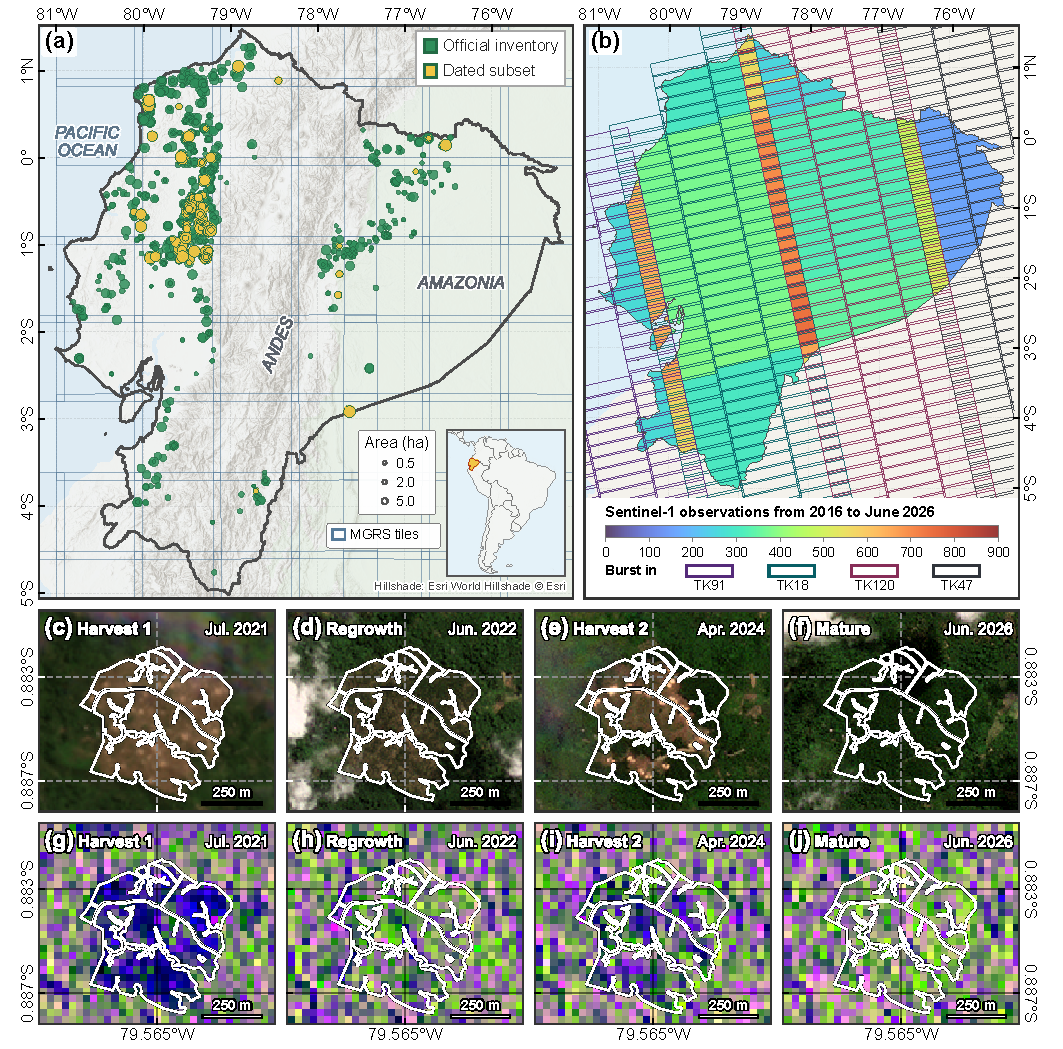
\includegraphics[width=0.96\linewidth]{figures/fig01_study_area.pdf}
    \caption{Study area and satellite observations of Ecuadorian balsa plantations. (a) Official balsa inventory and dated reference subset. (b) Cumulative ascending Sentinel-1 RTC burst observations (May 2016--June 2026) across tracks TK18, TK47, TK91, and TK120. (c--f) PlanetScope basemaps and (g--j) corresponding Sentinel-1 composites ($\mathrm{R}=\mathrm{VV}$, $\mathrm{G}=\mathrm{VH}$, $\mathrm{B}=\mathrm{VV}-\mathrm{VH}$) across two harvests and intervening regrowth.}
    \label{fig:study_area}
\end{figure}

% --------------------------------------------------------
\subsection{Satellite data}
\label{sec:satellitedata}

We compiled all dual-polarization (VV and VH) Sentinel-1 ascending-orbit acquisitions over mainland Ecuador from May 2016 to June 2026 (Fig.~\ref{fig:study_area}b) using Level-2 Radiometric Terrain Corrected backscatter products (RTC-S1) from NASA's OPERA project~\citep{opera2023rtc}. Each RTC-S1 product corresponds to a single Interferometric Wide-swath (IW) burst terrain-corrected with the Copernicus GLO-30 DEM, providing unfiltered $\gamma^{0}$ backscatter in linear power at 30~m spacing. Across four ascending relative-orbit tracks (TK18, TK47, TK91, and TK120; Table~\ref{tab:s1_observation_coverage}), 90,714 unique VV/VH burst acquisitions were organized onto Military Grid Reference System (MGRS) 30~m tiles using the S1-GRiTS framework (\url{https://github.com/ottoKae/S1-GRiTS}) to construct track-consistent monthly trajectories (Section~\ref{sec:s1_timeseries_representation}).

\begin{table*}[pos=!htbp]
    \centering
    \small
    \setlength{\tabcolsep}{4pt}
    \caption{Ascending Sentinel-1 OPERA RTC-S1 coverage over mainland Ecuador (May 2016--June 2026); monthly entries count stored tile--track months.}
    \label{tab:s1_observation_coverage}
    \begin{tabular*}{\linewidth}{@{\extracolsep{\fill}}llrrr@{}}
        \toprule
        Track family & Period & RTC bursts & Tile--track groups & Monthly entries \\
        \midrule
        TK18  & Sep. 2016--Jun. 2026 & 39,889 & 22 & 2,568 \\
        TK47  & Jun. 2016--Jun. 2026 & 8,839  & 7  & 525   \\
        TK91  & Oct. 2016--Jun. 2026 & 12,375 & 8  & 800   \\
        TK120 & May 2016--Jun. 2026 & 29,611 & 19 & 2,114 \\
        \midrule
        Total & May 2016--Jun. 2026 & \textbf{90,714} & 56 & \textbf{6,007} \\
        \bottomrule
    \end{tabular*}
\end{table*}

% --------------------------------------------------------
\subsection{Plantation inventory and reference harvest records}
\label{sec:reference_data}

Stand boundaries were obtained from Ecuador's 2025 national commercial plantation inventory (\texttt{FC001\_PLANTACION\_FORESTAL\_2025}), distributed by the Ministry of Agriculture and Livestock~\citep{MAGGeoportal}. Selecting field-validated balsa stands (species \texttt{BALSA} with status \texttt{VALIDADO}) yielded 3,498 polygons totalling 13,651.9~ha (Fig.~\ref{fig:study_area}a; Table~\ref{tab:inventory}). Smallholder-sized stands ($\leq 5$~ha) represented 77.5\% of polygon counts, whereas stands larger than 5~ha accounted for 70.3\% of total plantation area.

\begin{table*}[pos=!htbp]
    \centering
    \small
    \caption{Characteristics of the national balsa inventory and dated reference subset (medians [interquartile ranges] from 90~m Copernicus DEM~\citep{ESA2022CopernicusDEM} and 1~km CHELSA v2.1 normals~\citep{Karger2021CHELSAv21}).}
    \label{tab:inventory}
    \begin{tabular*}{\textwidth}{@{\extracolsep{\fill}}lrr@{}}
        \toprule
        Characteristic & Official inventory & Dated subset \\
        \midrule
        Stand count & 3,498 & 459 \\
        Total area (ha) & 13,651.9 & 2,302.6 \\
        Stand area (ha) & 1.7 [0.5--4.6] & 2.4 [0.9--5.6] \\
        \midrule
        Stands $\leq1$ ha, $n$ (\%) & 1,325 (37.9) & 122 (26.6) \\
        Stands $>1$--5 ha, $n$ (\%) & 1,385 (39.6) & 205 (44.7) \\
        Stands $>5$ ha, $n$ (\%) & 788 (22.5) & 132 (28.8) \\
        \midrule
        Elevation (m) & 183.7 [115.9--270.0] & 186.0 [146.6--222.9] \\
        Mean annual temperature ($^{\circ}$C) & 23.8 [23.3--24.5] & 23.3 [23.1--23.7] \\
        Annual precipitation (mm~yr$^{-1}$) & 2,908.9 [2,113.3--3,710.4] & 3,420.1 [3,127.3--3,739.3] \\
        \bottomrule
    \end{tabular*}
\end{table*}

To build an independent validation benchmark, we visually interpreted chronological PlanetScope monthly basemaps (${\sim}4.77$~m equatorial resolution~\citep{Planet2024Basemaps}) across inspected inventory stands, assigning each harvest event to the earliest month showing clear canopy removal (Fig.~\ref{fig:study_area}c--j). This yielded 1,049 month-dated reference harvest events across 459 stands during 2017--2025, of which 403 stands contained at least two recorded harvests (590 chronologically adjacent harvest pairs), providing direct multi-rotation reference histories despite occasional cloud-induced visibility delays.

% !TeX root = ../main.tex
\section{Methodology}
\label{sec:methods}

The framework reconstructs stand-level rotational harvest histories through three components: STS construction, pixelwise windowed CuSum detection, and stand-level harvest-history reconstruction (Fig.~\ref{fig:workflow}). First, STS construction organizes monthly Sentinel-1 observations into track-consistent trajectories at fixed 30~m grid cells (Section~\ref{sec:s1_timeseries_representation}). Second, windowed CuSum identifies persistent negative backscatter shifts using overlapping context windows, central decision intervals, and window-specific permutation testing (Section~\ref{sec:windowed_cusum}). Third, TDA consolidates staggered pixelwise detections into stand-level harvest events, while STP resolves spatial harvesting progression within individual events (Section~\ref{sec:stand_history_reconstruction}). Experimental design and accuracy assessment are described in Section~\ref{sec:experimental_evaluation}.

% Reconstructing rotational harvesting from decadal SAR records requires identifying successive stand-replacing canopy removals and resolving their spatial and temporal patterns. Three characteristics of short-rotation plantations guide our methodological design. First, harvesting recurs on the same land, requiring fixed spatial units across which successive management cycles can be tracked. Second, repeated harvesting and rapid regrowth continuously alter canopy structure, rendering a single long-term baseline inadequate for detecting subsequent harvests. Third, harvesting often progresses asynchronously within a stand over several months; collapsing a stand into a single averaged trajectory obscures this progression, whereas treating each pixel independently fragments a single harvest into multiple events.

% To address these requirements, we developed a four-stage framework (Fig.~\ref{fig:workflow}(a--d)): (1) organizing Sentinel-1 observations into track-consistent spatial time series (STS) at 30~m pixel locations; (2) detecting persistent negative backscatter shifts at the pixel level using windowed CuSum (Fig.~\ref{fig:workflow}(a, b)); (3) consolidating pixelwise detections into stand-level harvest events via temporal detection aggregation (TDA; Fig.~\ref{fig:workflow}(c)) while resolving intra-event harvesting progression via spatial timing partitioning (STP; Fig.~\ref{fig:workflow}(d)); and (4) evaluating event recovery and dating accuracy against independent reference records before mapping national harvest dynamics.

\begin{figure*}[pos=!htbp]
    \centering
    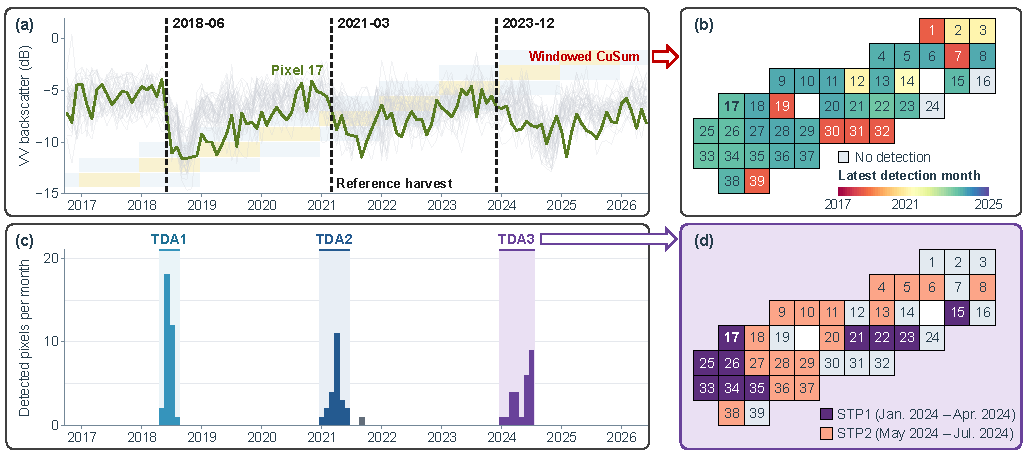
\includegraphics[width=\linewidth]{figures/fig02_workflow.pdf}
    \caption{Overview of the rotational harvest mapping framework, illustrated using inventory stand~22301. (a) Pixelwise windowed CuSum detection, showing 36-month context windows, 12-month decision intervals, and reference harvests. (b) Latest detection month per 30~m pixel during 2017--2025. (c) Three stand-level harvest events identified by temporal detection aggregation (TDA). (d) Intra-event timing groups identified by spatial timing partitioning (STP).}
    \label{fig:workflow}
\end{figure*}

% --------------------------------------------------
\subsection{Spatial time-series construction}
\label{sec:s1_timeseries_representation}

We represented each plantation stand as a spatially explicit set of long-term monthly pixelwise STS because harvesting recurs on the same land, requiring fixed spatial units across which successive management cycles can be tracked. Specifically, each STS links a track-consistent Sentinel-1 trajectory to a fixed 30~m grid cell~\citep{Guo2025SpatialAssociation} (Fig.~\ref{fig:sts_construction}(a--c)). Retaining individual pixel trajectories rather than averaging backscatter across stand polygons preserves both the temporal signatures of successive canopy changes and their spatial arrangement, providing the basis for subsequent pixelwise detection and stand-level harvest reconstruction.

\begin{figure*}[pos=!htbp]
    \centering
    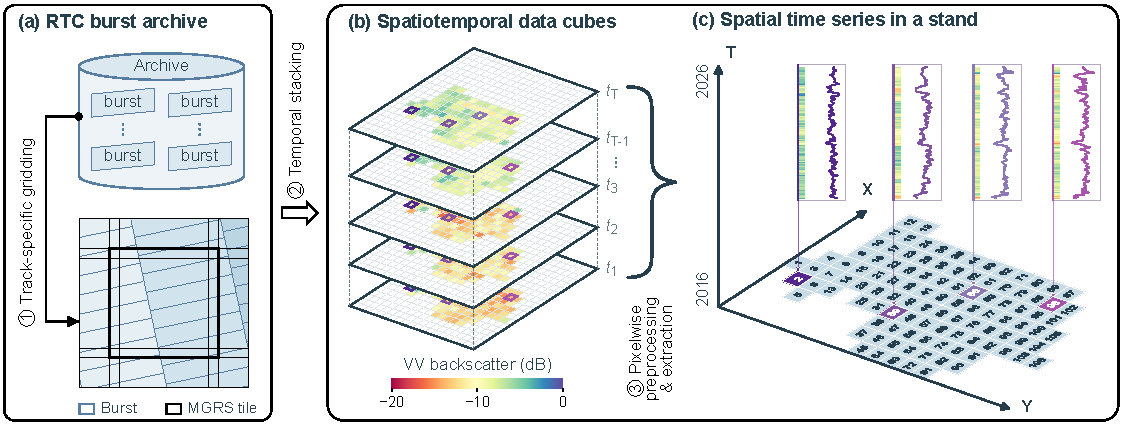
\includegraphics[width=\linewidth]{figures/fig03_sts_construction.pdf}
    \caption{Construction of 30~m spatial time series (STS) from Sentinel-1 RTC bursts. (a) RTC burst archive indexed to MGRS tiles by relative orbit (step~1). (b) Track-specific monthly spatiotemporal data cubes (step~2). (c) Pixelwise monthly VV trajectories extracted within stand polygons (step~3).}
    \label{fig:sts_construction}
\end{figure*}

Using the S1-GRiTS framework (Section~\ref{sec:satellitedata}), burst-level RTC-S1 images were organized by specific track on MGRS-aligned 30~m grids. For each grid cell and ascending track, valid linear-power $\gamma^{0}$ observations within each calendar month were summarized by their median and converted to decibels (dB). Maintaining each trajectory within a single relative orbit avoids mixing observations acquired under different viewing geometries~\citep{Navacchi2023RTCOrbit}. Where coverage from adjacent tracks or grid zones overlapped, the trajectory with the greatest number of jointly valid VV and VH months was retained at each location.

Grid cells whose centres fell within a plantation polygon were assigned to that stand. For stand $s$, this assignment defined a fixed set of $N_s$ pixels. All pixel trajectories were aligned to a uniform 126-month calendar from January 2016 to June 2026, with missing observations left unfilled. Monthly VV backscatter in dB, denoted $x_{u,t}$ for pixel $u$ and month $t$, served as the primary detection variable. VH was retained for polarization sensitivity analyses.

% --------------------------------------------------
\subsection{Pixelwise windowed CuSum detection}
\label{sec:windowed_cusum}

Repeated harvesting and rapid regrowth continuously alter canopy structure, rendering a single long-term baseline inadequate for detecting subsequent harvests. To address this challenge, we developed \textit{windowed CuSum}, a locally adaptive change-detection method for reconstructing recurrent harvest-related backscatter declines (Fig.~\ref{fig:windowed_cusum_concept}). It combines overlapping temporal contexts, non-overlapping decision intervals, and window-specific permutation testing. Overlapping windows renew local reference baselines as canopy conditions evolve across rotations, while central decision intervals assign candidate changes to distinct reporting periods. Window-specific permutation testing evaluates cumulative deviations against the temporal variability within each context window. Unlike recursive segmentation~\citep{Ygorra2023ReCuSum}, later detections do not depend on earlier detected change points.

\begin{figure*}[pos=!htbp]
    \centering
    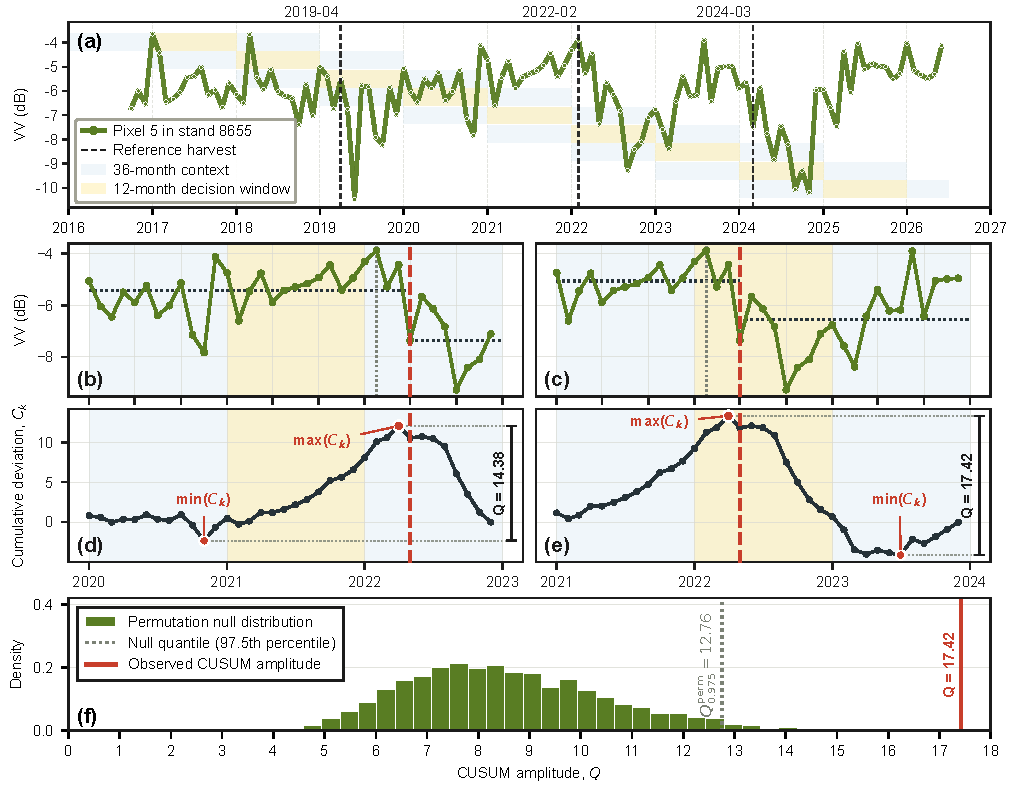
\includegraphics[width=\linewidth]{figures/fig04_windowed_cusum_concept.pdf}
    \caption{Principle of pixelwise windowed CuSum (Pixel~5, Stand~8655). (a) Monthly VV trajectory with overlapping 36-month context windows, central 12-month decision intervals, and reference harvests. (b,c) VV observations and pre-/post-shift means in two consecutive windows. (d,e) Cumulative deviations $C_k$ and full ranges $Q$, where the candidate falls outside the decision interval in (d) ($Q=14.38$) but enters testing in (e) ($Q=17.42$). (f) Permutation null distribution of $Q$, comparing observed $Q$ against the 97.5th percentile ($Q^{\mathrm{perm}}_{0.975}=12.76$).}
    \label{fig:windowed_cusum_concept}
\end{figure*}

We separated each context window $\mathcal{W}_j$ used for change estimation from its decision interval $\mathcal{D}_j$, within which candidates were eligible for reporting. As shown in Fig.~\ref{fig:windowed_cusum_concept}, the baseline used a 36-month context window ($W=36$), a central 12-month decision interval ($D=12$), and a 12-month advancement step ($S=12$). Each nominal window comprised the reporting year and its preceding and following years. Adjacent context windows therefore overlapped by 24 months, whereas decision intervals covered successive calendar years from 2017 to 2025 without overlap. The final context was truncated to January 2024--June 2026, retaining the full 2025 decision interval without shifting or padding the window. A window required at least 12 valid months under the joint VV--VH observation mask. All valid VV observations contributed to estimation in chronological order; missing months were not interpolated.

Within context window $\mathcal{W}_j$, let $t_1<\cdots<t_n$ denote the valid observation months for pixel $u$, with $z_i=x_{u,t_i}$ and $\bar z=n^{-1}\sum_{i=1}^{n}z_i$. We computed cumulative residuals and their full range as Equation~\eqref{eq:cusum_amplitude}.
\begin{equation}
    \begin{aligned}
        C_k &= \sum_{i=1}^{k}(z_i-\bar z),
        \qquad k=1,\ldots,n,\\
        Q &= \max_{1\leq k\leq n}C_k
             - \min_{1\leq k\leq n}C_k.
    \end{aligned}
    \label{eq:cusum_amplitude}
\end{equation}

A sustained decline produces predominantly positive deviations before the transition and negative deviations afterward, causing the cumulative sequence to rise and then fall. We selected its earliest global maximum and assigned the candidate date to the next valid observation month (Equation~\eqref{eq:candidate_date}). Thus, the candidate date denotes the first valid month after the cumulative peak, which need not be the next calendar month.
\begin{equation}
    \begin{aligned}
        k^* &=
        \min\left\{
            k\in\{1,\ldots,n\}:
            C_k=\max_{1\leq \ell\leq n}C_\ell
        \right\},\\
        \hat{\tau}_{u,j} &= t_{k^*+1},
        \qquad k^*<n.
    \end{aligned}
    \label{eq:candidate_date}
\end{equation}


A candidate proceeded to permutation testing only when $k^*<n$, $\hat{\tau}_{u,j}\in\mathcal{D}_j$, and $\bar z_{\mathrm{post}}<\bar z_{\mathrm{pre}}$. Here, $\bar z_{\mathrm{pre}}$ and $\bar z_{\mathrm{post}}$ are the means of $z_1,\ldots,z_{k^*}$ and $z_{k^*+1},\ldots,z_n$, respectively. Windows failing these conditions were skipped without searching for alternative peaks. For each qualifying window, we randomly reordered its $n$ valid values $B$ times and recomputed the CUSUM range:
\begin{equation}
    p_{\mathrm{perm}}
    =
    \frac{
        1+\sum_{b=1}^{B}
        \mathbf{1}\!\left\{
            Q_b^{\mathrm{perm}}\geq Q
        \right\}
    }{B+1},
    \label{eq:permutation_pvalue}
\end{equation}
where $Q_b^{\mathrm{perm}}$ is the CUSUM range computed from the $b$th permuted sequence and $\mathbf{1}\{\cdot\}$ is the indicator function~\citep{PhipsonSmyth2010Permutation}. This comparison evaluates the observed CUSUM range against a window-specific random-order distribution, rather than testing the candidate date itself. Permuted sequences were used only to recompute $Q$; candidate-date and directional screening were not repeated.

We initially used $B=3{,}999$ permutations, refining the total to $19{,}999$ when the initial $p_{\mathrm{perm}}\in[0.015,0.035]$ to improve precision near the acceptance threshold. Candidates were accepted when the final $p_{\mathrm{perm}}\leq\alpha_{\mathrm{ts}}$, with $\alpha_{\mathrm{ts}}=0.025$. This threshold applies to individual candidate windows and does not specify a record-wide false-alarm rate. Unrestricted permutation assumes exchangeability under the null and does not preserve temporal autocorrelation; sensitivity to this assumption was examined using calendar-block permutations (Section~\ref{sec:experimental_evaluation}). Selecting one candidate per window and using non-overlapping annual decision intervals allowed at most one accepted detection per pixel per reporting year. Detections in successive years were retained to reconstruct recurrent harvesting.

% ---------------------------------------------------------------------------
\subsection{Stand-level event aggregation and harvest-history mapping}
\label{sec:stand_history_reconstruction}

Harvesting often progresses asynchronously within a stand over several months. Collapsing a stand into a single averaged trajectory obscures this progression, whereas treating each pixel independently fragments a single harvest into multiple detections. In our framework, TDA consolidates staggered pixelwise detections into stand-level harvest events, while STP resolves the spatial organization of harvesting progression within each event (Fig.~\ref{fig:workflow}(c, d)).
% Harvest-history statistics were derived from TDA events; STP did not alter their number or representative dates.

For stand $s$ and month $t$, $A_{s,t}$ denotes the number of distinct pixels with accepted detections, and $V_{s,t}$ counts pixels with valid monthly inputs and context windows containing at least 12 valid months. Given the fixed stand pixel count $N_s$, monthly states were classified as shown in Equation~\eqref{eq:monthly_activity_state}.
\begin{equation}
    \mathrm{State}_{s,t} =
    \begin{cases}
        \text{active}, & A_{s,t}\geq 1,\\
        \text{observed non-detection}, & A_{s,t}=0,\; V_{s,t}\geq 0.5N_s,\\
        \text{unknown}, & \text{otherwise}.
    \end{cases}
    \label{eq:monthly_activity_state}
\end{equation}

Consecutive active months were grouped and merged across a single observed non-detection month. At least two consecutive observed non-detection months separated events; gaps containing unknown months without this separation remained unresolved. Components adjoining unresolved internal boundaries were not reported. The remaining components were retained as harvest events when distinct contributing pixels accounted for at least 20\% of $N_s$, including events censored at the observation-period edges. Each event was dated by the median of its contributing pixel--month detections, rounded to the nearest month. Repeated detections from the same pixel contributed to event dating but counted only once toward spatial support.

STP tested events with $N_s\geq25$ and at least 15 distinct contributing pixels. Spatial testing used the tile--track group with the most contributing pixels, requiring at least four pixels and three edge-sharing neighbour pairs. Within this group, neighbours were linked when their first-detection months differed by at most $\delta\in\{0,1,2\}$ months; connected components defined initial timing zones. For each tolerance, $J_\delta$ counted neighbour pairs crossing zone boundaries. We permuted first-detection months among fixed pixel locations 999 times, rebuilding zones at every tolerance for each permutation. The resulting counts $J_{\delta,b}$ supplied the null mean $\mu_\delta$ and standard deviation $\sigma_\delta$ in Equation~\eqref{eq:spatial_organization}.
\begin{equation}
    \begin{aligned}
        T_{\mathrm{obs}} &= \min_{\delta\in\{0,1,2\}} \frac{J_\delta-\mu_\delta}{\sigma_\delta},\\
        T_b &= \min_{\delta\in\{0,1,2\}} \frac{J_{\delta,b}-\mu_\delta}{\sigma_\delta},\\
        p_{\mathrm{sp}} &= \frac{1+\sum_{b=1}^{999}\mathbf{1}\!\left\{T_b\leq T_{\mathrm{obs}}\right\}}{1000}.
    \end{aligned}
    \label{eq:spatial_organization}
\end{equation}

Thus, observed and permuted statistics included the same tolerance search. Partitioning required positive null standard deviations at all tolerances, $T_{\mathrm{obs}}<0$, and $p_{\mathrm{sp}}\leq0.05$.

At the selected tolerance, zones with fewer than three pixels were merged into the temporally nearest larger zone based on median first-detection months. Zones were then ordered by their rounded median first-detection months and divided into timing groups at gaps exceeding two months. Partitions were retained only when at least two groups each contained at least 20\% of $N_s$; otherwise, the event remained unsplit. Group representative months followed the TDA dating rule, while the parent event's date remained unchanged.

Stand harvest frequency was the number of TDA events during 2017--2025. Annual and quarterly counts used representative event months, whereas inter-harvest intervals were measured between consecutive events' first-detection months. Counts were aggregated by canton, and intervals within each 10-km hexagon were summarized by their modal three-month bin, with ties flagged separately. Interval distributions were also compared across 1-km K\"oppen--Geiger climate zones~\citep{Beck2023KoppenGeiger}.


% =========================================================
\subsection{Experimental design and accuracy assessment}
\label{sec:experimental_evaluation}

We evaluated harvest-associated SAR backscatter responses, stand-level event detection and rotational-history recovery, component contributions and configuration sensitivity, and performance against alternative detectors. The reference catalogue comprised 1,049 dated harvest events across 459 stands during 2017--2025.

To characterize backscatter responses, observations were aligned to each reference harvest month (month $0$). Pixels were eligible if they had at least six valid observations in both VV and VH during months $-12$ to $-3$ and at least two during months $0$ to $+2$. For each eligible pixel, backscatter change was calculated as the post-harvest median minus the pre-harvest median. Reference events with eligible pixels covering at least 50\% of the stand's fixed membership were retained, yielding 978 events. Pixelwise changes were summarized by their median within each event, and event-aligned trajectories were summarized over months $-12$ to $+12$ relative to pre-harvest baselines. Pooled monthly backscatter observations from the plantation inventory provided distributional context. Uncertainty in event-level responses was estimated using 5,000 bootstrap resamples of 61 spatial blocks.

All detector configurations were evaluated using the same TDA and reference-matching rules. Within each stand, a detected event matched a reference harvest if its first-to-last detection span overlapped the reference month $\pm1$ month. One-to-one assignment maximized the number of matches. Precision, recall, and F1 were calculated from counts pooled across the 459 reference stands as shown in Equation~\eqref{eq:reference_agreement_metrics}.
\begin{equation}
    \begin{aligned}
        P_{\mathrm{ref}} &= \frac{M}{N_{\mathrm{det}}}, \qquad
        R_{\mathrm{ref}} = \frac{M}{N_{\mathrm{ref}}},\\
        F_{1,\mathrm{ref}} &= \frac{2M}{N_{\mathrm{det}}+N_{\mathrm{ref}}},
    \end{aligned}
    \label{eq:reference_agreement_metrics}
\end{equation}
where $M$ is the number of matched events, $N_{\mathrm{det}}$ the number of detected events, and $N_{\mathrm{ref}}$ the number of reference harvests. Because optical interpretation may miss cloud-obscured harvests, these metrics quantify agreement with documented reference records.

Multi-rotation recovery was assessed using the 590 chronologically adjacent reference harvest pairs, counting a pair as recovered only when both harvests matched distinct detected events in Equation~\eqref{eq:reference_pair_retention}.
\begin{equation}
    R_{\mathrm{pair}}
    =
    \frac{
        \sum_s\sum_{k=1}^{n_s-1} m_{s,k}m_{s,k+1}
    }{
        \sum_s(n_s-1)
    },
    \label{eq:reference_pair_retention}
\end{equation}
where $n_s$ is the number of reference harvests in stand $s$ and $m_{s,k}$ equals one if its $k$th harvest was matched and zero otherwise. Dating accuracy was measured as the mean absolute error (MAE) between representative detection months and reference months. Pairwise MAE comparisons used the same reference events successfully matched by both methods.

Progressive ablation measured the incremental effect of adding overlapping context windows ($W=36$, $S=12$), central decision intervals ($D=12$), negative-shift screening, and permutation testing ($\alpha_{\mathrm{ts}}=0.025$) to a single full-record CuSum. Configuration sensitivity was assessed relative to the baseline ($W=36$, $D=S=12$, VV, $\alpha_{\mathrm{ts}}=0.025$). We varied context length ($W=24,48,60$ months), decision interval and stride ($(D,S)=(12,6)$ and $(6,6)$), and polarization (VH, VV--VH union, and intersection requiring agreement within $\pm2$ months). Additional configurations combined $W=24$ with $D=S=6$. We also varied $\alpha_{\mathrm{ts}}$ across $\{0.005,0.01,0.025,0.05,0.10\}$ and tested 3--6-month calendar-block permutations that retained within-block temporal order to assess sensitivity to temporal dependence.

Windowed CuSum was benchmarked against 13 alternative detector configurations: maximum monthly decline; classical lower CuSum~\citep{Page1954CUSUM}; raw and decrease-filtered monthly CuSum NRT~\citep{Ygorra2024CuSumNRT}; raw, decrease-filtered, and first-post adaptations of recursive ReCuSum~\citep{Ygorra2023ReCuSum}; a dual-polarization Bayesian online change detection (BOCD) prototype~\citep{Bottani2026f-pol_BOCD}; original and expanded CCDC configurations~\citep{Zhu2014CCDC,Bullock2022CCDC_S1}; structural-change breakpoints; BFAST Monitor~\citep{Verbesselt2012BFASTMonitor}; and EWMACD~\citep{Brooks2014EWMACD}. All configurations used the same spatial support and monthly observation series, with polarization inputs appropriate to each method. Between-configuration F1 differences were assessed using 5,000 paired stand-level bootstrap resamples, drawing the same stands for each configuration and recalculating pooled F1. Percentile confidence intervals were 97.5\% for the two primary Bonferroni-adjusted contrasts against raw monthly CuSum NRT and original CCDC, and 95\% for other comparisons. MAE differences on shared matches were assessed using paired stand-level bootstrap resampling. Detailed detector settings and implementation rules are provided in the accompanying repository (Data and code availability).

% !TeX root = ../main.tex
\section{Results}
\label{sec:results}

% --------------------------------------------------------
\subsection{Sentinel-1 backscatter responses to harvest events}
\label{sec:s1_signatures}

Across the 978 reference harvest events meeting the paired VV--VH coverage requirements, harvesting consistently reduced C-band backscatter in both polarizations, even though pooled pre- and post-harvest backscatter distributions overlapped substantially (Fig.~\ref{fig:s1_population_signatures}a). Median VV backscatter declined from $-6.00$~dB before harvesting (months $-12$ to $-3$) to $-7.51$~dB immediately afterward (months $0$ to $+2$), while median VH declined from $-12.54$ to $-13.98$~dB. Within individual stands, however, paired post-minus-pre changes were negative in 97.3\% of events for VV and 95.0\% for VH, with median declines of $-1.45$~dB (95\% CI: $-1.64$ to $-1.24$~dB) and $-1.40$~dB (95\% CI: $-1.60$ to $-1.19$~dB), respectively (Fig.~\ref{fig:s1_population_signatures}b).

\begin{figure*}[pos=!htbp]
    \centering
    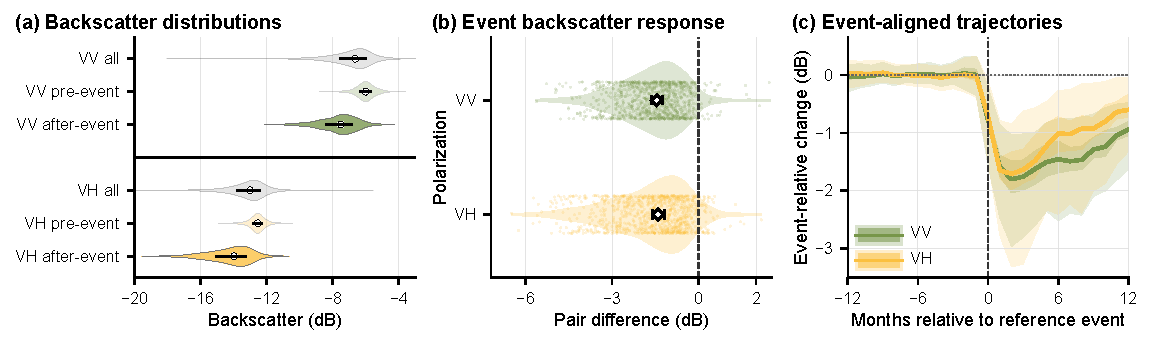
\includegraphics[width=\linewidth]{figures/fig05_backscatter_signatures.pdf}
    \caption{Sentinel-1 VV and VH backscatter responses across 978 reference harvests. (a) Pre-event ($-12$ to $-3$ months), after-event ($0$ to $+2$ months), and inventory-wide (all) monthly backscatter distributions (medians and IQRs). (b) Paired post-minus-pre differences within events (medians and 95\% CIs). (c) Event-aligned relative backscatter trajectories with IQRs (light shading) and 95\% spatial-block bootstrap CIs (dark shading).}
    \label{fig:s1_population_signatures}
\end{figure*}

Event-aligned trajectories showed sharp backscatter drops at harvesting followed by gradual recovery during early stand regrowth (Fig.~\ref{fig:s1_population_signatures}c). Median deviations reached their minimum at month $+2$ ($-1.80$~dB for VV and $-1.71$~dB for VH) and subsequently converged toward pre-harvest baselines. Across the 950 events with complete 12-month post-harvest coverage, median deviations remained negative at month $+12$ ($-0.94$~dB for VV and $-0.60$~dB for VH), with pointwise 95\% confidence intervals remaining below zero from month $0$ through month $+12$ in both polarizations.

% --------------------------------------------------------
\subsection{Component contributions and configuration sensitivity}
\label{sec:cusum_components_sensitivity}

\subsubsection{Contributions of local context and candidate screening}
\label{sec:representation_component_ablation}

Progressive component ablation demonstrated that local context windows provide the sensitivity needed to capture repeated harvests, whereas central decision-interval admission and permutation testing establish precision (Table~\ref{tab:component_ablation}). Evaluating each pixel trajectory with a single full-record CuSum yielded high precision ($0.810$) but missed nearly half of all documented harvests ($R_{\mathrm{ref}}=0.531$, $F_{1,\mathrm{ref}}=0.641$), recovering only 18.0\% (106/590) of chronologically adjacent reference harvest pairs. Replacing the full-record baseline with overlapping 36-month local windows raised recall to $0.952$ (999/1,049 events) and adjacent-pair recovery to 93.4\% (551/590), but unscreened repeated searches inflated stand-level detected events from 688 to 2,327, lowering precision to $0.429$ ($\Delta F_{1,\mathrm{ref}}=-0.050$).

\begin{table*}[pos=!htbp]
    \centering
    \small
    \setlength{\tabcolsep}{4pt}
    \caption{Progressive component ablation of windowed CuSum across 459 reference stands (1,049 harvests). $N_{\mathrm{det}}$ and $M$ denote detected stand-level events and matched harvests; $\Delta F_{1,\mathrm{ref}}$ compares each row with its predecessor (95\% bootstrap CIs). Bold marks column maxima.}
    \label{tab:component_ablation}
    \begin{tabular*}{\linewidth}{@{\extracolsep{\fill}}lrrrrrc@{}}
        \toprule
        Cumulative configuration &
        $N_{\mathrm{det}}$ &
        $M$ &
        $P_{\mathrm{ref}}$ &
        $R_{\mathrm{ref}}$ &
        $F_{1,\mathrm{ref}}$ &
        $\Delta F_{1,\mathrm{ref}}$ (95\% CI) \\
        \midrule
        Full-record CuSum
        & 688 & 557 & \textbf{0.810} & 0.531 & 0.641 & -- \\
        + Local windows
        & 2,327 & 999 & 0.429 & \textbf{0.952} & 0.592 & $-0.050$ [$-0.075$, $-0.022$] \\
        + Decision-interval admission
        & 1,843 & 992 & 0.538 & 0.946 & 0.686 & $+0.094$ [$+0.081$, $+0.107$] \\
        + Negative-direction screening
        & 1,843 & 992 & 0.538 & 0.946 & 0.686 & $\phantom{+}0.000$ [$\phantom{+}0.000$, $\phantom{+}0.000$] \\
        + Permutation screening
        & 1,208 & 945 & 0.782 & 0.901 & \textbf{0.837} & $+0.151$ [$+0.134$, $+0.169$] \\
        \bottomrule
    \end{tabular*}
\end{table*}

Restricting candidate admission to the central 12-month decision interval eliminated 484 boundary-induced events while forfeiting only seven matched harvests, lifting $F_{1,\mathrm{ref}}$ to $0.686$ ($\Delta F_{1,\mathrm{ref}}=+0.094$). Because localizing candidates at the global cumulative residual maximum already selected downward shifts across all 79,301 admitted pixel--month candidates, explicit negative-direction screening left detections unchanged ($\Delta F_{1,\mathrm{ref}}=0.000$). Finally, window-specific permutation testing ($\alpha_{\mathrm{ts}}=0.025$) removed 635 low-confidence events while retaining 945 matched harvests, raising precision to $0.782$ and $F_{1,\mathrm{ref}}$ to $0.837$ ($\Delta F_{1,\mathrm{ref}}=+0.151$). The complete configuration recovered 83.9\% (495/590) of adjacent reference pairs and produced compact stand-level events with a median detection span of four months (with 6.4\%, or 77 events, exceeding 12 months).

\subsubsection{Configuration sensitivity of windowed CuSum}
\label{sec:cusum_configuration_sensitivity}

Detection performance remained stable across moderate variations in window length and search schedule, while showing clear sensitivity to polarization choice and block-permutation length (Table~\ref{tab:cusum_configuration_sensitivity}). Shortening the context window to $W=24$ months slightly increased precision ($0.808$) and yielded an $F_{1,\mathrm{ref}}$ of $0.848$ ($\Delta F_{1,\mathrm{ref}}=+0.010$, 95\% CI: $-0.004$ to $+0.025$), though with fewer matched harvests (935 vs.\ 945) and adjacent pairs (486/590 vs.\ 495/590) than the $W=36$ baseline. Conversely, extending the window to $W=48$ and $W=60$ months progressively reduced recall ($0.860$ and $0.823$) and adjacent-pair recovery (452/590 and 407/590), lowering $F_{1,\mathrm{ref}}$ to $0.820$ at $W=60$ ($\Delta F_{1,\mathrm{ref}}=-0.017$). Halving the search stride ($D=12, S=6$) or both interval and stride ($D=S=6$) produced $F_{1,\mathrm{ref}}$ values nearly indistinguishable from the annual baseline ($0.834$ and $0.840$; paired differences within $\pm0.004$, with 95\% CIs spanning zero), recovering 518/590 and 487/590 adjacent pairs with median event spans of five and four months, respectively. Combining $W=24$ with $D=S=6$ similarly yielded $F_{1,\mathrm{ref}}=0.843$ ($\Delta F_{1,\mathrm{ref}}=+0.005$, 95\% CI: $-0.007$ to $+0.018$).

\begin{table*}[pos=!htbp]
    \centering\small
    \setlength{\tabcolsep}{3pt}
    \caption{Configuration sensitivity of windowed CuSum relative to the baseline (VV, $W=36$, $D=S=12$ months, $\alpha_{\mathrm{ts}}=0.025$). $\Delta F_{1,\mathrm{ref}}$ shows differences from baseline (95\% bootstrap CIs). Bold marks column maxima.}
    \label{tab:cusum_configuration_sensitivity}
    \begin{tabular*}{\linewidth}{@{\extracolsep{\fill}}lrrrrrc@{}}
        \toprule
        Configuration & $N_{\mathrm{det}}$ & $M$ & $P_{\mathrm{ref}}$ & $R_{\mathrm{ref}}$ & $F_{1,\mathrm{ref}}$ & $\Delta F_{1,\mathrm{ref}}$ (95\% CI) \\
        \midrule
        Baseline ($W=36$, $D=S=12$, VV) & 1,208 & 945 & 0.782 & 0.901 & 0.837 & -- \\
        \midrule
        \multicolumn{7}{@{}l}{\textit{Context length ($D=S=12$)}} \\
        $W=24$ months & 1,157 & 935 & 0.808 & 0.891 & \textbf{0.848} & $+0.010$ [$-0.004$, $+0.025$] \\
        $W=48$ months & 1,120 & 902 & 0.805 & 0.860 & 0.832 & $-0.006$ [$-0.018$, $+0.006$] \\
        $W=60$ months & 1,056 & 863 & 0.817 & 0.823 & 0.820 & $-0.017$ [$-0.033$, $-0.002$] \\
        \midrule
        \multicolumn{7}{@{}l}{\textit{Search schedule ($W=36$)}} \\
        $D=12$, $S=6$ months & 1,273 & 968 & 0.760 & 0.923 & 0.834 & $-0.004$ [$-0.011$, $+0.005$] \\
        $D=S=6$ months & 1,188 & 940 & 0.791 & 0.896 & 0.840 & $+0.003$ [$-0.006$, $+0.012$] \\
        \midrule
        \multicolumn{7}{@{}l}{\textit{Polarization ($W=36$, $D=S=12$)}} \\
        VH & 1,127 & 852 & 0.756 & 0.812 & 0.783 & $-0.054$ [$-0.072$, $-0.036$] \\
        VV--VH union & 1,430 & 976 & 0.683 & \textbf{0.930} & 0.787 & $-0.050$ [$-0.061$, $-0.038$] \\
        VV--VH intersection & 809 & 737 & \textbf{0.911} & 0.703 & 0.793 & $-0.044$ [$-0.064$, $-0.025$] \\
        \bottomrule
    \end{tabular*}
\end{table*}

Among polarization strategies, VV alone outperformed VH ($F_{1,\mathrm{ref}}=0.783$, $\Delta F_{1,\mathrm{ref}}=-0.054$) as well as dual-polarization fusion: taking the VV--VH union raised recall to $0.930$ at the expense of precision ($0.683$, $F_{1,\mathrm{ref}}=0.787$; and $0.807$ vs.\ $0.843$ under $W=24, D=S=6$), whereas requiring $\pm2$-month VV--VH agreement raised precision to $0.911$ but depressed recall to $0.703$ ($F_{1,\mathrm{ref}}=0.793$). Varying the permutation threshold across $\alpha_{\mathrm{ts}}\in[0.005,0.10]$ kept $F_{1,\mathrm{ref}}$ within $0.804\text{--}0.847$, peaking at $\alpha_{\mathrm{ts}}=0.01$ ($\Delta F_{1,\mathrm{ref}}=+0.009$, 95\% CI: $-0.001$ to $+0.019$). In contrast, replacing independent shuffling with calendar-block permutations of 3, 4, 5, and 6 months sharply curtailed sensitivity within the 36-month window, reducing recall to $0.647$, $0.397$, $0.090$, and $0.015$ and $F_{1,\mathrm{ref}}$ to $0.744$, $0.550$, $0.163$, and $0.030$, respectively.

% --------------------------------------------------------
\subsection{Benchmark performance against alternative detectors}
\label{sec:benchmark_null_sensitivity}

Windowed CuSum achieved the highest overall accuracy ($F_{1,\mathrm{ref}}=0.837$) among all 14 evaluated detector configurations (Table~\ref{tab:benchmark_comparison}). In the two primary Bonferroni-adjusted contrasts, windowed CuSum outperformed raw monthly CuSum NRT by $+0.253$ in $F_{1,\mathrm{ref}}$ (97.5\% CI: $0.230$ to $0.275$) and the original CCDC configuration by $+0.103$ (97.5\% CI: $0.076$ to $0.133$). Extreme operating points emerged among specialized alternatives: decrease-filtered monthly CuSum NRT achieved the highest recall ($0.939$, 985/1,049 events) but generated 1,960 stand-level events ($P_{\mathrm{ref}}=0.503$, $F_{1,\mathrm{ref}}=0.655$), with a median event span of seven months (and 32.6\% of events exceeding 12 months for raw NRT), whereas the dual-polarization BOCD prototype achieved the highest precision ($0.888$) at the cost of missing four-fifths of reference harvests ($R_{\mathrm{ref}}=0.197$).

\begin{table*}[pos=!htbp]
    \centering
    \small
    \setlength{\tabcolsep}{4pt}
    \caption{Benchmark comparison of 14 detector configurations across 459 reference stands (1,049 harvests) under identical TDA rules. Bold marks column maxima.}
    \label{tab:benchmark_comparison}
    \begin{tabular*}{\linewidth}{@{\extracolsep{\fill}}lrrrrr@{}}
        \toprule
        Detector configuration & $N_{\mathrm{det}}$ & $M$ & $P_{\mathrm{ref}}$ & $R_{\mathrm{ref}}$ & $F_{1,\mathrm{ref}}$ \\
        \midrule
        Windowed CuSum (Ours) & 1,208 & 945 & 0.782 & 0.901 & \textbf{0.837} \\
        Maximum monthly decline & 2,470 & 691 & 0.280 & 0.659 & 0.393 \\
        Classical lower CuSum & 1,254 & 317 & 0.253 & 0.302 & 0.275 \\
        BOCD prototype (VV+VH) & 233 & 207 & \textbf{0.888} & 0.197 & 0.323 \\
        Monthly CuSum NRT (raw) & 2,159 & 938 & 0.434 & 0.894 & 0.585 \\
        Monthly CuSum NRT (decrease-filtered) & 1,960 & 985 & 0.503 & \textbf{0.939} & 0.655 \\
        ReCuSum (decrease-filtered) & 946 & 763 & 0.807 & 0.727 & 0.765 \\
        ReCuSum (raw) & 1,688 & 716 & 0.424 & 0.683 & 0.523 \\
        ReCuSum first-post adaptation & 1,024 & 818 & 0.799 & 0.780 & 0.789 \\
        CCDC original configuration & 953 & 735 & 0.771 & 0.701 & 0.734 \\
        CCDC expanded configuration & 825 & 659 & 0.799 & 0.628 & 0.703 \\
        Structural breakpoints & 902 & 729 & 0.808 & 0.695 & 0.747 \\
        BFAST Monitor adaptation & 773 & 207 & 0.268 & 0.197 & 0.227 \\
        EWMACD adaptation & 1,135 & 473 & 0.417 & 0.451 & 0.433 \\
        \bottomrule
    \end{tabular*}
\end{table*}

The strongest external competitor was the first-post adaptation of recursive ReCuSum ($F_{1,\mathrm{ref}}=0.789$), over which windowed CuSum gained $+0.048$ in $F_{1,\mathrm{ref}}$ (95\% CI: $0.032$ to $0.065$). While both methods maintained comparable precision ($0.782$ vs.\ $0.799$), identical median event spans (four months; 6.4\% vs.\ 5.3\% exceeding 12 months), and virtually identical dating accuracy across 804 shared matches (representative-month MAE of $0.803$ vs.\ $0.799$ months; paired difference $+0.005$ months, 95\% CI: $-0.039$ to $+0.048$), windowed CuSum substantially improved multi-rotation completeness, lifting single-event recall from 78.0\% to 90.1\% and adjacent-pair recovery from 65.6\% (387/590) to 83.9\% (495/590).

% --------------------------------------------------------
\subsection{Mapping rotational harvesting across mainland Ecuador}
\label{sec:harvest_mapping}

\subsubsection{Stand-level harvest histories and intra-event progression}
\label{sec:mapping_stand_histories}

At the local scale, TDA consolidated pixelwise detections into discrete rotational harvest sequences across 15 representative stands during 2017--2025, identifying 34 stand-level events (one to three harvests per stand; Fig.~\ref{fig:harvest_mapping_stands}a,b,d,e,g,h). For instance, Stand~716 underwent two harvests centred in June 2021 and April 2024, whereas Stand~22301 completed three harvest cycles centred in June 2018, April 2021, and June 2024.

\begin{figure*}[pos=!htbp]
    \centering
    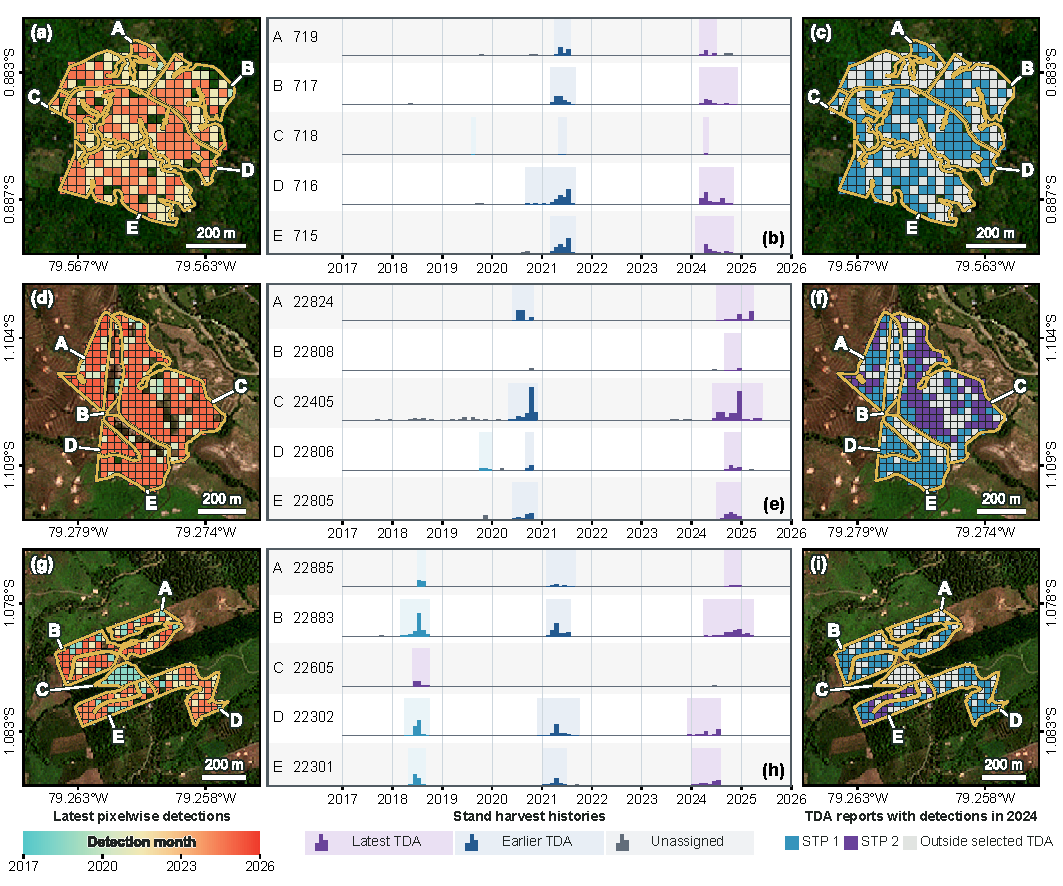
\includegraphics[width=\linewidth]{figures/fig06_stand_harvest_histories.pdf}
    \caption{Stand-level harvest histories and intra-event progression across three balsa neighbourhoods (March 2025 PlanetScope basemaps). (a,d,g) Latest pixelwise detection months (2017--2025). (b,e,h) Monthly detected-pixel counts (bars) and TDA event spans (shading; latest vs.\ earlier events). (c,f,i) Intra-event timing groups (STP~1 and STP~2) within complete TDA events containing 2024 detections. Letters (A--E) link stands across panels in each row.}
    \label{fig:harvest_mapping_stands}
\end{figure*}

Where harvesting progressed gradually across large management units, STP resolved distinct spatial felling stages within individual stand-level events without inflating stand harvest counts (Fig.~\ref{fig:harvest_mapping_stands}c,f,i). In Stand~22405, 109 of 156 pixels detected between June 2024 and May 2025 separated into two spatially coherent sub-blocks of 33 and 76 pixels centred in August and December 2024, respectively (Fig.~\ref{fig:harvest_mapping_stands}e,f). Similarly, in Stand~22301, pixels active between January and July 2024 partitioned into sub-blocks of 10 and 16 pixels centred in March and July 2024 (Fig.~\ref{fig:harvest_mapping_stands}h,i). Across the entire national inventory, STP identified significant spatial progression in 70 of the 2,125 size-eligible detected events, partitioning them into 142 intra-event timing groups.

\subsubsection{National harvesting hotspots, temporal pulses, and recurrence intervals}
\label{sec:mapping_national_recurrence}

Applying the framework across mainland Ecuador's balsa inventory (3,364 evaluable stands out of 3,498; 134 small polygons lacked 30~m grid-centre support) identified 6,303 stand-level harvest events across 2,931 stands during 2017--2025 (Fig.~\ref{fig:harvest_mapping_national}). Whereas 433 evaluable stands showed no harvest detection and 926 experienced a single harvest, 2,005 stands (59.6\%) underwent two or more harvests, confirming widespread multi-rotation management over the nine-year window.

\begin{figure*}[pos=!htbp]
    \centering
    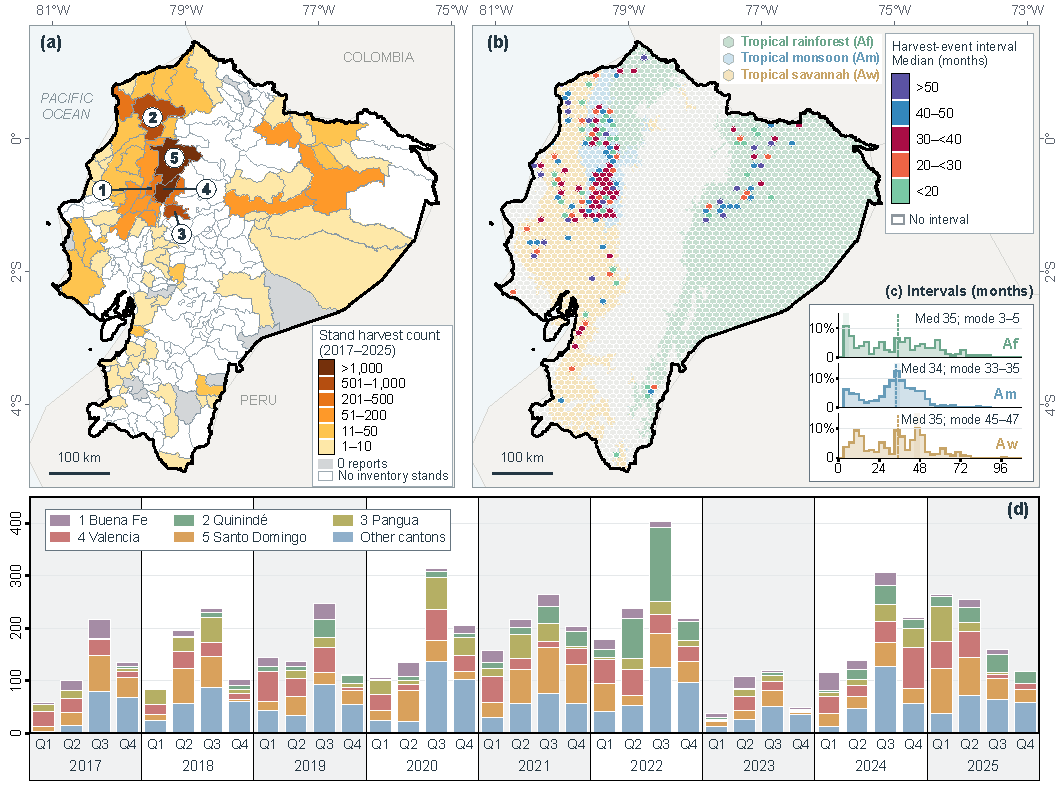
\includegraphics[width=\linewidth,height=0.74\textheight,keepaspectratio]{figures/fig07_national_harvest_patterns.pdf}
    \caption{National balsa harvest patterns in mainland Ecuador, 2017--2025. (a) Cumulative stand-level harvest counts by canton. (b) Modal inter-harvest intervals (3-month bins) in 10-km hexagons over K\"oppen--Geiger climate zones. (c) Inter-harvest interval distributions in Af, Am, and Aw climates (dashed lines: medians; purple bars: modal bins). (d) Quarterly stand-level harvest counts by canton.}
    \label{fig:harvest_mapping_national}
\end{figure*}

Cumulative harvest activity was strongly concentrated along the western coastal lowland and foothill plantation belt, delineating Ecuador's core production hotspots (Fig.~\ref{fig:harvest_mapping_national}a): five cantons---Santo Domingo (1,358 events), Valencia (1,076), Pangua (684), Quinind\'e (670), and Buena Fe (475)---accounted for 67.6\% (4,263/6,303) of all detected harvests nationwide. Temporally, harvesting exhibited a pronounced industry-wide cycle rather than a steady annual rate (Fig.~\ref{fig:harvest_mapping_national}d). Annual harvest events rose to a peak of 1,037 in 2022---culminating in the third quarter of 2022 with 403 events, including 141 in Quinind\'e alone---before dropping sharply to 315 in 2023 and rebounding to 781 in 2024 and 795 in 2025.

Across the 2,005 repeatedly harvested stands, consecutive stand-level events defined 3,372 inter-harvest intervals (measured between successive first-detection months), yielding a national median interval of 34 months (IQR: 22--43 months) and a dominant modal bin of 33--35 months (Fig.~\ref{fig:harvest_mapping_national}b,c). This national distribution was anchored by the tropical monsoon (Am) zone, which contained 84.8\% of all intervals ($n=2{,}861$), sharing the same 34-month median, 33--35 month mode, and a compact IQR of 24--42 months. Tropical savannah (Aw; $n=345$, 10.2\%) and tropical rainforest (Af; $n=150$, 4.4\%) stands exhibited nearly identical medians (35 months each) but wider dispersion and contrasting modal peaks: Aw shifted toward a longer modal bin of 45--47 months (IQR: 14--47 months), whereas the small Af sample peaked at 3--5 months alongside a broad IQR of 14.25--50 months.

% !TeX root = ../main.tex
\section{Discussion}
\label{sec:discussion}

% --------------------------------------------------------
\subsection{Adaptive detection of recurrent plantation harvests}
\label{sec:discussion_local_adaptation}

Recurrent harvest detection depends on changes relative to evolving canopy conditions. Although pooled pre- and post-harvest backscatter distributions overlapped, within-event trajectories showed a consistent decline followed by recovery. Temporal trajectories therefore provide information that static backscatter thresholds cannot capture. Similar post-harvest responses have been reported in other short-rotation plantations~\citep{Spracklen2021Acacia}. VV also supported better event detection than VH despite comparable median declines, indicating that harvest contrast alone does not determine detection performance. Background variability during regrowth may also affect the separation of harvest signals from other fluctuations~\citep{Sabir2024AdaptiveCuSUM}.

Over successive rotations, a full-record baseline combines different stages of stand development~\citep{Kennedy2010LandTrendr}. Windowed CuSum renews this baseline locally, while central decision intervals and permutation testing constrain candidate acceptance. Unlike recursive ReCuSum~\citep{Ygorra2023ReCuSum}, later searches do not depend on earlier segmentation decisions. This distinction matters when an early harvest is missed or misdated. The retrospective design also uses temporal context beyond the candidate event, unlike methods intended for immediate disturbance alerts~\citep{Ygorra2024CuSumNRT}.

The comparison with first-post ReCuSum shows that the main gain was more complete harvest histories, with similar dating accuracy on shared detections. Recovering successive events on the same land is essential for estimating harvest frequency and recurrence intervals; accurately dating isolated events alone cannot provide this information.

% --------------------------------------------------------
\subsection{Interpreting balsa harvest dynamics, hotspots, and recurrence intervals}
\label{sec:discussion_harvest_histories}

Harvest operations can span several months and spatial sub-blocks, creating a mismatch between pixelwise changes and management events. TDA addresses this mismatch by consolidating detections while distinguishing observed inactivity from insufficient observation support. STP adds spatial detail within those events. Together, they support interpretation at both the stand and sub-stand scales without treating each harvesting stage as another rotation.

The national reconstruction adds a temporal dimension to the plantation inventory, identifying where harvesting recurs and when activity concentrates. The western concentration and the 2022 peak followed by a sharp decline reveal substantial spatial and temporal variation in canopy turnover. These patterns can guide comparisons with timber production and planting records; the satellite histories alone do not establish market demand as their cause.

The national median interval of 34 months is consistent with balsa reaching commercial dimensions within approximately three years on productive sites~\citep{GonzalezOsorio2010Balsa,CanadasLopez2019BalsaGrowth}. However, the dominance of Am plantations means that this national estimate primarily describes that climate zone. The longer modal interval in Aw plantations may reflect slower growth under seasonal water limitation~\citep{Yuan2026BalsaWaterUse}, although management differences could also contribute. The 3--5-month mode in the smaller Af sample cannot represent a complete biological rotation; possible explanations include staged clearing and non-harvest backscatter changes. These intervals describe detected stand-level canopy turnover and need not equal planting-to-harvest rotation lengths.

% --------------------------------------------------------
\subsection{Limitations, transferability, and future perspectives}
\label{sec:discussion_limitations}

C-band backscatter changes do not uniquely identify clear-felling. Rainfall, flooding, windthrow, and thinning can produce declines~\citep{Doblas2020Rainfall}, while residual trees or slash can weaken harvest signals~\citep{Balling2023Texture}. Optical reference records may also omit cloud-obscured events, so unmatched detections can include undocumented harvests as well as false detections. Field or production records would help distinguish these outcomes.

Spatial support and temporal assumptions further limit interpretation. The 30~m grid and stand-support threshold can omit small or narrow cuts. Permutation testing assumes exchangeable observations; the sharp loss of recall under calendar-block permutations shows that temporal dependence materially affects detection. This sensitivity requires further evaluation rather than treating the nominal threshold as a guaranteed false-alarm rate. Dependence on post-event observations also makes the framework most suitable for retrospective reconstruction, with reduced temporal support near the archive endpoint.

Transfer to other short-rotation plantations, including \textit{Eucalyptus} and \textit{Acacia}~\citep{Spracklen2021Acacia,Huang2026EucalyptusAge}, would require evaluating harvest responses and adapting temporal windows to local growth and management. Future work could combine complementary SAR frequencies with independent harvest records to distinguish canopy removal from moisture-driven changes and assess recovery across successive rotations.
% !TeX root = ../main.tex
\section{Conclusion}
\label{sec:conclusion}

We developed the windowed CuSum detector to reconstruct recurrent harvest histories in short-rotation plantations from decadal Sentinel-1 observations. The detector re-estimates reference levels within local temporal windows to assess negative backscatter changes against evolving growth and recovery backgrounds. Spatiotemporal aggregation then consolidates accepted pixelwise detections into stand-level harvest reports. Windowed CuSum achieved the highest reference F1 score of 0.837 among the 14 evaluated detector configurations. Compared with the first-post ReCuSum adaptation, it recovered more reference harvest events and adjacent reference-event pairs. Application to the mapped balsa inventory in Ecuador revealed a concentration of harvest reports in western cantons. The median interval between successive stand-level reports was 34 months. Spatial timing partitioning characterized variation in detection timing within individual reports. The resulting histories provide a spatially explicit basis for examining plantation canopy turnover and integrating satellite observations with independent management and production records.

% !TeX root = ../main.tex
\section*{Declaration of competing interest}
The authors declare that they have no known competing financial interests or personal relationships that could have appeared to influence the work reported in this paper.

\section*{Data and code availability}
The stand boundaries, dated harvest references, monthly Sentinel-1 time series, and pixelwise detection and stand-level aggregation outputs are archived on Zenodo as dataset version 1.0.0 (\url{https://doi.org/10.5281/zenodo.24223182}) under the CC BY-NC-SA 4.0 licence.

Sentinel-1 OPERA Level-2 RTC-S1 products are publicly available from the NASA Alaska Satellite Facility Distributed Active Archive Center (\url{https://search.asf.alaska.edu/}), and the Ecuadorian commercial forest plantation inventory (\texttt{FC001\_PLANTACION\_FORESTAL\_2025}) is publicly accessible via the Geoportal del Agro Ecuatoriano. The S1-GRiTS spatial time-series toolkit is available at \url{https://github.com/ottoKae/S1-GRiTS}. The windowed CuSum source code, benchmark parameter configurations, and aggregated stand-level harvest summary tables are publicly available in the project repository (to be archived on Zenodo upon acceptance); commercial PlanetScope basemap imagery cannot be redistributed due to licensing terms.

\section*{Funding}
This work was supported by the Startup Research Fund of Henan Academy of Sciences (Grant No.~242025005) and the Open Research Fund Program of the MNR Key Laboratory for Geo-Environmental Monitoring of the Great Bay Area.

\section*{Declaration of generative AI and AI-assisted technologies in the writing process}
During the preparation of this work, the authors used large language model tools to assist with code refactoring and English language polishing. After using these tools, the authors reviewed and edited the content as needed and take full responsibility for the content of the published article.


\printcredits
\bibliographystyle{cas-model2-names}
\bibliography{references}

\end{document}
